\documentclass[aspectratio=169,10pt]{beamer}

% =========================================================
% THEME & STYLING (ICACT 2026 IEEE 16:9 BLUE THEME)
% =========================================================
\usetheme{Madrid}
\usecolortheme{default}

% IEEE / ICACT Theme Colors
\definecolor{ieeeBlue}{RGB}{0, 102, 153}     % #006699
\definecolor{ieeeDarkBlue}{RGB}{0, 51, 102}  % #003366
\definecolor{alertRed}{RGB}{204, 0, 0}
\definecolor{highlightGreen}{RGB}{0, 136, 68}
\definecolor{bgGray}{RGB}{245, 247, 250}

\setbeamercolor{palette primary}{bg=ieeeDarkBlue, fg=white}
\setbeamercolor{palette secondary}{bg=ieeeBlue, fg=white}
\setbeamercolor{palette tertiary}{bg=ieeeBlue!80, fg=white}
\setbeamercolor{title}{bg=ieeeBlue, fg=white}
\setbeamercolor{frametitle}{bg=ieeeBlue, fg=white}
\setbeamercolor{structure}{fg=ieeeBlue}
\setbeamercolor{block title}{bg=ieeeBlue!15, fg=ieeeDarkBlue}
\setbeamercolor{block body}{bg=ieeeBlue!5, fg=black}

% Remove default navigation symbols
\setbeamertemplate{navigation symbols}{}

% Custom Footline matching template
\setbeamertemplate{footline}{
  \leavevmode%
  \hbox{%
  \begin{beamercolorbox}[wd=.75\paperwidth,ht=2.5ex,dp=1ex,left,leftskip=1em]{author in head/foot}%
    \tiny\color{gray} ICACT 2026 $\bullet$ IEEE Conference Record No. 70625 $\bullet$ 1--2 September 2026 $\bullet$ Online
  \end{beamercolorbox}%
  \begin{beamercolorbox}[wd=.25\paperwidth,ht=2.5ex,dp=1ex,right,rightskip=1em]{title in head/foot}%
    \tiny\color{gray} Paper ID: [Paper ID] \hspace{1em} \insertframenumber{} / \inserttotalframenumber
  \end{beamercolorbox}}%
  \vskip0pt%
}

% Packages
\usepackage{amsmath,amssymb}
\usepackage{booktabs}
\usepackage{tikz}
\usetikzlibrary{shapes.geometric, arrows.meta, positioning, fit, calc}
\usepackage{pgfplots}
\pgfplotsset{compat=1.18}

% =========================================================
% PRESENTATION METADATA
% =========================================================
\title[NLOS Acoustic Sensing via Spectral Gating]{\textbf{NLOS Acoustic Sensing via Spectral Gating and GCC-PHAT}}

\author[P. Narendra et al.]{
  \textbf{Polisetti Narendra}$^{1,*}$, \textbf{Vijaya Raju Motru}$^{1}$, \textbf{Suresh Kumar Sreedharan}$^{1}$, \\
  \textbf{Praveena Mallampalli}$^{1}$, \textbf{T Murali Mohan}$^{1}$, \textbf{T V Satyasheela}$^{1}$
}

\institute[SCET]{
  $^{1}$\scriptsize Department of Computer Science and Engineering,\\
  Swarnandhra College of Engineering \& Technology (Autonomous), Narsapur, Andhra Pradesh, India\\[0.3em]
  \textbf{Presenting Author:} Polisetti Narendra ($^*$narendresh@yahoo.com)
}

\date[\textbf{ICACT 2026}]{\small 2026 IEEE 3rd International Conference on Advanced Computing Technologies (ICACT 2026)\\September 1--2, 2026}

% =========================================================
% DOCUMENT
% =========================================================
\begin{document}

% ---------------------------------------------------------
% SLIDE 1: TITLE SLIDE (0:30)
% ---------------------------------------------------------
\begin{frame}[plain]
  \begin{tikzpicture}[remember picture, overlay]
    \fill[ieeeBlue] (current page.north west) rectangle ([yshift=-2cm]current page.north east);
    \node[anchor=north west, text=white, font=\bfseries\large] at ([xshift=0.8cm, yshift=-0.5cm]current page.north west) {ICACT 2026};
    \node[anchor=north west, text=white!90, font=\tiny] at ([xshift=0.8cm, yshift=-1.1cm]current page.north west) {2026 IEEE 3rd International Conference on Advanced Computing Technologies};
    \node[anchor=north west, text=white!80, font=\tiny] at ([xshift=0.8cm, yshift=-1.4cm]current page.north west) {IEEE Conference Record No. 70625 $\bullet$ 1--2 September 2026 $\bullet$ Online $\bullet$ Technically Co-Sponsored by IEEE Nepal Section};
    \node[anchor=north east, text=white, font=\bfseries\normalsize] at ([xshift=-0.8cm, yshift=-0.8cm]current page.north east) {IEEE};
  \end{tikzpicture}
  \vspace{1.2cm}
  
  \begin{center}
    {\Large\color{ieeeDarkBlue}\textbf{NLOS Acoustic Sensing via Spectral Gating and GCC-PHAT}}\\[0.5em]
    \small \textbf{Polisetti Narendra}$^{1,*}$, \textbf{Vijaya Raju Motru}$^{1}$, \textbf{Suresh Kumar Sreedharan}$^{1}$, \\
    \textbf{Praveena Mallampalli}$^{1}$, \textbf{T Murali Mohan}$^{1}$, \textbf{T V Satyasheela}$^{1}$\\[0.4em]
    \tiny $^{1}$Department of Computer Science and Engineering, Swarnandhra College of Engineering \& Technology (Autonomous), Narsapur, AP, India\\
    \tiny \textbf{Presenting Author:} Polisetti Narendra (\texttt{narendresh@yahoo.com})
  \end{center}
  
  \vfill
  \tiny\centering \textbf{Paper ID:} [Your Paper ID] $\bullet$ \textbf{Session:} [Session Name] $\bullet$ \textbf{Time:} 10:00 AM (10 Min Talk + 2 Min Q\&A)
\end{frame}

% ---------------------------------------------------------
% SLIDE 2: 1. INTRODUCTION AND MOTIVATION (1:30)
% ---------------------------------------------------------
\begin{frame}{1. Introduction and Motivation \hfill {\small\color{gray}1 min 30 s}}
\begin{itemize}
    \setlength{\itemsep}{0.6em}
    \item \textbf{The Core Problem: Spatial Blindness in Indoor Vision:} \\
    Surveillance cameras are fundamentally constrained by line-of-sight (LOS) geometry. Structural corners, L-shaped corridor bends, and partitions create permanent visual blind spots where optical detection cannot perceive critical safety anomalies in time.
    
    \item \textbf{The Physics Opportunity (Acoustic Diffraction \& Reflection):}
    \begin{itemize}
        \item Unlike light, acoustic waves diffract around sharp geometric edges and reflect off rigid corridor surfaces (walls, floors, ceilings), naturally propagating beyond visual obstructions.
        \item Non-Line-of-Sight (NLOS) awareness is achieved via \textbf{wave mechanics}, not optical imaging.
    \end{itemize}
    
    \item \textbf{The Breakdown of Current Deep Learning Audio Approaches:}
    \begin{itemize}
        \item State-of-the-art Audio Spectrogram Transformers (AST / PANNs) require multi-second context buffers ($>1000$~ms structural latency), heavy RAM ($>200$~MB), and continuous raw audio retention, violating sub-150~ms emergency response budgets and raising severe privacy concerns.
    \end{itemize}
    
    \item \textbf{The Central Thesis of Our Paper:} \\
    \textit{\textbf{Deterministic, physics-driven signal-processing pipelines can reliably detect impulsive NLOS anomalies under reverberant corridor conditions with bounded latency ($<120$~ms) and zero raw audio persistence.}}
\end{itemize}
\end{frame}

% ---------------------------------------------------------
% SLIDE 3: 2. RELATED WORK AND THE GAP (1:00)
% ---------------------------------------------------------
\begin{frame}{2. Related Work and the Research Gap \hfill {\small\color{gray}1 min 00 s}}
\begin{itemize}
    \setlength{\itemsep}{0.8em}
    \item \textbf{Paradigm A: Deep Learning Semantic AED (AST, PANNs, CNNs):}
    \begin{itemize}
        \item \textit{Strengths:} High semantic categorization accuracy on public benchmarks (FSD50K).
        \item \textit{Fatal Flaw in Edge Safety:} Multi-second temporal buffering introduces $>1000$~ms latency; massive memory footprints ($>85\text{M}$ params) overwhelm lightweight edge MCUs/ARM nodes without NPUs.
    \end{itemize}
    
    \item \textbf{Paradigm B: Classical Source Localization in Reverberation:}
    \begin{itemize}
        \item \textit{Amplitude Thresholding:} Completely fails in corridors; benign door slams and footsteps exceed thresholds, creating massive false alarms.
        \item \textit{Steered Response Power (SRP-PHAT):} Accurate but computationally prohibitive for edge micro-arrays due to 3D spatial grid searching.
        \item \textit{Standard Cross-Correlation (TDOA):} Degrades severely under multipath echoes where delayed reflections obscure the direct path.
    \end{itemize}
    
    \item \textbf{The Specific Gap Addressed in This Work:} \\
    \textbf{Deterministic, Zero-Persistence Signal Discrimination:} Designing a lightweight two-stage filter (spectral gating $\delta$ + autocorrelation periodicity $\rho$) combined with GCC-PHAT in a formalized reverberant operational regime ($\mathcal{R}_{rev}$).
\end{itemize}
\end{frame}

% ---------------------------------------------------------
% SLIDE 4: 3. PROPOSED METHOD (2:30)
% ---------------------------------------------------------
\begin{frame}{3. Proposed Method: Deterministic NLOS Acoustic Sensor \hfill {\small\color{gray}2 min 30 s}}
\textbf{The Core Idea:} \textit{Differentiate chaotic impulses from mechanical noise using physical spectral-temporal signatures, estimate direction via GCC-PHAT, and immediately overwrite raw PCM audio.}

\vspace{0.4em}
\begin{center}
\resizebox{0.95\textwidth}{!}{
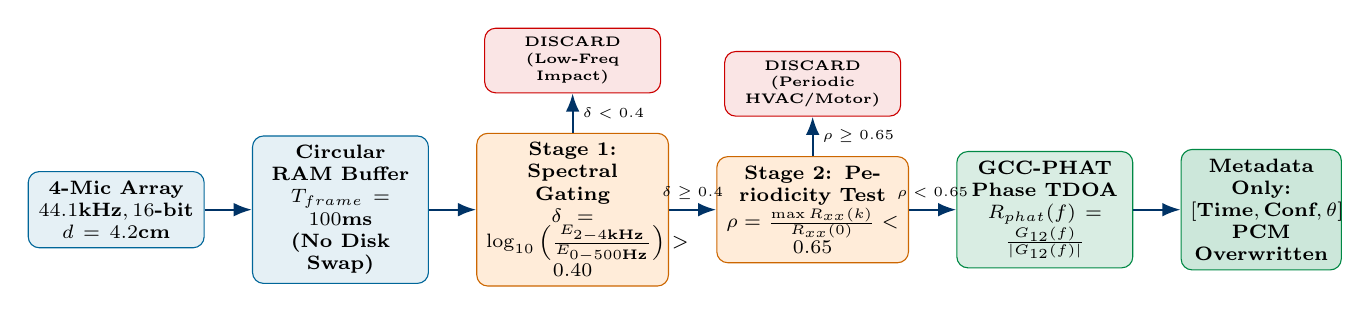
\begin{tikzpicture}[node distance=1.1cm, auto]
    \tikzset{
        box/.style={rectangle, draw=ieeeBlue, fill=ieeeBlue!10, text centered, rounded corners, minimum height=0.9cm, font=\scriptsize\bfseries},
        gate/.style={rectangle, draw=orange!80!black, fill=orange!15, text centered, rounded corners, minimum height=0.9cm, font=\scriptsize\bfseries},
        reject/.style={rectangle, draw=alertRed, fill=alertRed!10, text centered, rounded corners, minimum height=0.7cm, font=\tiny\bfseries},
        pass/.style={rectangle, draw=highlightGreen, fill=highlightGreen!15, text centered, rounded corners, minimum height=0.9cm, font=\scriptsize\bfseries},
        arrow/.style={draw=ieeeDarkBlue, -Latex, thick}
    }
    \node [box, text width=2.0cm] (mic) {4-Mic Array\\$44.1\text{kHz}, 16\text{-bit}$\\$d=4.2\text{cm}$};
    \node [box, right=0.6cm of mic, text width=2.0cm] (ring) {Circular RAM Buffer\\$T_{frame}=100\text{ms}$\\(No Disk Swap)};
    \node [gate, right=0.6cm of ring, text width=2.2cm] (stft) {Stage 1: Spectral Gating\\$\delta = \log_{10}\left(\frac{E_{2-4\text{kHz}}}{E_{0-500\text{Hz}}}\right) > 0.40$};
    \node [reject, above=0.5cm of stft, text width=2.0cm] (rej1) {DISCARD\\(Low-Freq Impact)};
    \node [gate, right=0.6cm of stft, text width=2.2cm] (auto) {Stage 2: Periodicity Test\\$\rho = \frac{\max R_{xx}(k)}{R_{xx}(0)} < 0.65$};
    \node [reject, above=0.5cm of auto, text width=2.0cm] (rej2) {DISCARD\\(Periodic HVAC/Motor)};
    \node [pass, right=0.6cm of auto, text width=2.0cm] (gcc) {GCC-PHAT Phase TDOA\\$R_{phat}(f) = \frac{G_{12}(f)}{|G_{12}(f)|}$};
    \node [box, right=0.6cm of gcc, text width=1.8cm, fill=highlightGreen!20, draw=highlightGreen] (out) {Metadata Only:\\$[\text{Time}, \text{Conf}, \theta]$\\PCM Overwritten};

    \draw [arrow] (mic) -- (ring);
    \draw [arrow] (ring) -- (stft);
    \draw [arrow] (stft) -- node[right, font=\tiny]{$\delta < 0.4$} (rej1);
    \draw [arrow] (stft) -- node[above, font=\tiny]{$\delta \ge 0.4$} (auto);
    \draw [arrow] (auto) -- node[right, font=\tiny]{$\rho \ge 0.65$} (rej2);
    \draw [arrow] (auto) -- node[above, font=\tiny]{$\rho < 0.65$} (gcc);
    \draw [arrow] (gcc) -- (out);
\end{tikzpicture}
}
\end{center}

\vspace{-0.3em}
\begin{columns}[T]
\column{0.5\textwidth}
\textbf{Two-Stage Physical Discrimination:}
\begin{itemize}
    \scriptsize
    \item \textbf{Spectral Gating ($\delta > 0.40$):} Compares 2--4~kHz impulsive energy against 0--500~Hz rumble ($>2.5\times$ energy ratio).
    \item \textbf{Periodicity Rejection ($\rho < 0.65$):} Autocorrelation excludes repeating mechanical cycles (HVAC/fans, $k_{min} \approx 120\text{Hz}$).
\end{itemize}
\column{0.5\textwidth}
\textbf{Deterministic Reverberant Localization:}
\begin{itemize}
    \scriptsize
    \item \textbf{GCC-PHAT Normalization:} Magnitude whitening eliminates echo dominance, extracting phase delays for Azimuth ($\theta$).
    \item \textbf{Privacy by Design:} Raw audio is wiped immediately upon feature extraction; only 3-tuple telemetry is emitted.
\end{itemize}
\end{columns}
\end{frame}

% ---------------------------------------------------------
% SLIDE 5: 4. EXPERIMENTAL SETUP (1:00)
% ---------------------------------------------------------
\begin{frame}{4. Experimental Setup \& Testbed \hfill {\small\color{gray}1 min 00 s}}
\begin{columns}[T]
\column{0.48\textwidth}
\begin{block}{\textbf{Corridor Physical Testbed}}
\scriptsize
\begin{itemize}
    \item \textbf{Geometry:} L-shaped academic corridor ($2.4\text{m} \times 3.0\text{m} \times 30\text{m}$).
    \item \textbf{Acoustic Profile:} $RT_{60} \approx 1.2\text{ s}$, Critical Distance $D_c \approx 2.1\text{ m}$.
    \item \textbf{Operating Regime $\mathcal{R}_{rev}$:} Operational envelope ($S_{env} = 15\text{m}$) $\gg D_c$, deliberately testing multipath-dominant physics.
    \item \textbf{Hardware Array:} 4-mic linear array, spacing $d = 4.2\text{cm}$ ($f_{alias} = 4083\text{Hz} > 4\text{kHz}$ band limit).
\end{itemize}
\end{block}

\column{0.48\textwidth}
\begin{block}{\textbf{Comprehensive Evaluation Dataset}}
\scriptsize
\begin{itemize}
    \item \textbf{Hybrid Corpus ($\sim 1000$ Events):}
    \begin{itemize}
        \tiny
        \item 500 Impulsive Vocal Screams (FSD50K $\otimes$ RIR)
        \item 200 Glass Break Incidents (MIVIA $\otimes$ RIR)
        \item 150 Heavy Door Slams (Synthesized $\otimes$ RIR)
        \item 12 Hours Physical Ambient HVAC Hum
        \item 4 Hours Physical Campus Footsteps
    \end{itemize}
    \item \textbf{Hardware Test Platform:} Quad-Core ARM Cortex-A72 ($1.5\text{GHz}$), single-stream PCM ring buffer.
\end{itemize}
\end{block}
\end{columns}

\vspace{0.4em}
\begin{block}{\textbf{Strict Latency Budget Specification}}
\centering\footnotesize
$T_{frame} (100\text{ms}) + T_{proc} (18\text{ms}) = \mathbf{T_{total} < 120\text{\textbf{ ms}}}$ (Quad-Core ARM CPU Utilization $<15\%$)
\end{block}
\end{frame}

% ---------------------------------------------------------
% SLIDE 6: 5. RESULTS AND EMPIRICAL FINDINGS (2:30)
% ---------------------------------------------------------
\begin{frame}{5. Results and Empirical Findings \hfill {\small\color{gray}2 min 30 s}}
\begin{columns}[T]
\column{0.50\textwidth}
\textbf{1. NLOS Safety Envelope Detection ($100\text{dB}$ Source):}
\vspace{0.2em}
\resizebox{\columnwidth}{!}{
\begin{tabular}{lcc}
\toprule
\textbf{NLOS Distance} & \textbf{Visual Camera} & \textbf{Proposed Acoustic} \\
\midrule
5 Meters  & 0.0\% (Occluded) & \textbf{100.0\%} ($n=20$) \\
15 Meters ($S_{env}$) & 0.0\% (Occluded) & \textbf{100.0\%} ($n=20$) \\
25 Meters & 0.0\% (Occluded) & \textbf{89.0\%} ($n=20$) \\
35 Meters & 0.0\% (Occluded) & \textbf{57.0\%} ($n=20$) \\
\bottomrule
\end{tabular}
}
\tiny Result: Perfect $100\%$ detection maintained within the $15\text{m}$ safety zone.

\vspace{0.5em}
\textbf{2. Ablation on Filtering Heuristics:}
\vspace{0.2em}
\resizebox{\columnwidth}{!}{
\begin{tabular}{lcc}
\toprule
\textbf{Active Pipeline Configuration} & \textbf{Recall} & \textbf{False Pos. Rate} \\
\midrule
SPL Volume Trigger Only & 99.5\% & 42.6\% (Unusable) \\
+ Log Spectral Gate ($\delta > 0.4$) & 96.0\% & 8.2\% \\
\textbf{+ Periodic Rejection ($\rho < 0.65$) (Full)} & \textbf{94.5\%} & \textbf{1.8\% ($24\times$ drop!)} \\
\bottomrule
\end{tabular}
}

\column{0.48\textwidth}
\textbf{3. Physical Spectral Energy Discrimination:}
\vspace{0.1em}
\begin{center}
\resizebox{0.92\columnwidth}{!}{
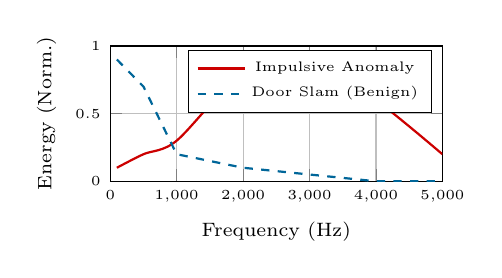
\begin{tikzpicture}
    \begin{axis}[
        width=5.8cm, height=3.3cm,
        xlabel={\scriptsize Frequency (Hz)}, ylabel={\scriptsize Energy (Norm.)},
        xmin=0, xmax=5000, ymin=0, ymax=1.0,
        xtick={0, 1000, 2000, 3000, 4000, 5000}, ytick={0, 0.5, 1.0},
        legend pos=north east, legend style={font=\tiny},
        grid=major, tick label style={font=\tiny}, label style={font=\scriptsize}
    ]
    \addplot[color=alertRed, thick, smooth] coordinates {
        (100,0.1)(500,0.2)(1000,0.3)(2000,0.8)(3000,0.9)(4000,0.6)(5000,0.2)
    };
    \addlegendentry{Impulsive Anomaly}
    \addplot[color=ieeeBlue, thick, dashed] coordinates {
        (100,0.9)(500,0.7)(1000,0.2)(2000,0.1)(3000,0.05)(4000,0.0)(5000,0.0)
    };
    \addlegendentry{Door Slam (Benign)}
    \end{axis}
\end{tikzpicture}
}
\end{center}
\vspace{-0.6em}
\tiny \textbf{SNR Robustness:} At $60\text{dB}$ ambient traffic noise, pipeline maintains \textbf{98.2\% Precision, 94.5\% Recall, 96.3\% F1}.
\end{columns}
\end{frame}

% ---------------------------------------------------------
% SLIDE 7: DISCUSSION AND LIMITATIONS (OPTIONAL)
% ---------------------------------------------------------
\begin{frame}{Discussion and Architectural Trade-offs \hfill {\small\color{gray}Optional}}
\begin{columns}[T]
\column{0.48\textwidth}
\begin{block}{\textbf{Why Deterministic Processing Wins}}
\scriptsize
\begin{itemize}
    \item \textbf{Latency Boundedness:} Pure $O(N \log N)$ FFT operations guarantee $<120\text{ms}$ reaction time without GPU acceleration.
    \item \textbf{Privacy by Architectural Restriction:} The sensing node physically cannot record conversations or run speech-to-text; raw audio is immediately erased from volatile RAM ring buffers.
    \item \textbf{Lightweight Network Telemetry:} Generates small 3-tuple metadata packets, preventing campus network congestion.
\end{itemize}
\end{block}

\column{0.48\textwidth}
\begin{block}{\textbf{Physical \& Operational Limitations}}
\scriptsize
\begin{itemize}
    \item \textbf{Azimuth-Only Localization:} Linear 4-mic array resolves horizontal angle ($\theta$) only; multi-floor elevation requires planar/volumetric arrays.
    \item \textbf{Multipath Jitter in Metallic Corridors:} Severe reflections induce up to $\pm 8^\circ$ angular drift.
    \item \textbf{Crowd Noise Masking:} Dense crowd chatter ($70\text{dB}$) masks the 2--4~kHz band, reducing recall to $78.0\%$.
    \item \textbf{Corridor-Specific Tuning:} Thresholds ($\delta, \rho$) assume reflective indoor acoustics ($\alpha \approx 0.05$--$0.1$).
\end{itemize}
\end{block}
\end{columns}

\vspace{0.4em}
\begin{center}
\footnotesize \textbf{System Role:} Operates strictly as a \textbf{first-responder physical trigger} that cues PTZ cameras and security personnel to occluded hotspots in real time.
\end{center}
\end{frame}

% ---------------------------------------------------------
% SLIDE 8: 6. CONCLUSION AND FUTURE WORK (1:00)
% ---------------------------------------------------------
\begin{frame}{6. Conclusion and Future Roadmap \hfill {\small\color{gray}1 min 00 s}}
\begin{itemize}
    \setlength{\itemsep}{0.8em}
    \item \textbf{What We Set Out to Do:} \\
    Eliminate blind spots in indoor corridor safety monitoring where line-of-sight cameras fail, without incurring the high latency, heavy compute, and privacy risks of deep learning audio transformers.
    
    \item \textbf{The Core Takeaway (One Sentence to Remember):} \\
    \textit{\textbf{Deterministic, physics-driven acoustic signal processing extends spatial awareness into visually occluded corridors, achieving $>95\%$ detection within a $15\text{m}$ envelope, $<120\text{ms}$ latency, $1.8\%$ false alarms, and zero audio storage.}}
    
    \item \textbf{Future Research Roadmap:}
    \begin{itemize}
        \item \textbf{Volumetric Array Geometries:} Extending microphone arrays to 3D tetrahedral configurations for simultaneous 3D azimuth and elevation localization in stairwells.
        \item \textbf{Adaptive Dynamic Thresholding:} Employing ambient noise tracking to dynamically adapt spectral ratio $\delta$ under variable occupancy and crowd density.
        \item \textbf{Cross-Modal Triggering in ScholarMaster Engine:} Coupling acoustic directional vectors with automated PTZ camera pan-tilt steering for instantaneous visual confirmation.
    \end{itemize}
\end{itemize}
\end{frame}

% ---------------------------------------------------------
% SLIDE 9: REFERENCES AND DECLARATIONS
% ---------------------------------------------------------
\begin{frame}{References and Declarations \hfill {\small\color{gray}Shown Only}}
\begin{columns}[T]
\column{0.65\textwidth}
\textbf{Key References:}
\tiny
\begin{enumerate}
    \item \textbf{C. Knapp and G. Carter}, "The generalized correlation method for estimation of time delay," \textit{IEEE Trans. ASSP}, 1976.
    \item \textbf{J. B. Allen and D. A. Berkley}, "Image method for efficiently simulating small-room acoustics," \textit{J. Acoust. Soc. Am.}, 1979.
    \item \textbf{G. Valenzise et al.}, "Scream and gunshot detection and localization for audio-surveillance systems," in \textit{Proc. IEEE AVSS}, 2007.
    \item \textbf{J. H. DiBiase}, "A high-accuracy closed-form approximation to SRP-PHAT and TDOA," \textit{Proc. IEEE ICASSP}, 2000.
    \item \textbf{P. Narendra et al.}, ``Memory-Bound Edge Efficiency Envelope (MBEEE): A Hardware-Level Analytical Model,'' \textit{Journal for Basic Sciences}, vol. 26, no. 5, pp. 31--37, 2026.
\end{enumerate}

\column{0.33\textwidth}
\textbf{Declarations:}
\tiny
\begin{itemize}
    \item \textbf{Data \& Ethics:} Uses public benchmark datasets (FSD50K, MIVIA) combined with room impulse response (RIR) spatial convolutions.
    \item \textbf{Reproducibility:} Deterministic signal equations, filter thresholds, and hardware array geometries fully documented.
    \item \textbf{Funding / Acknowledgements:} None received (conducted solely and independently by the authors without external funding).
    \item \textbf{Conflicts of Interest:} None declared.
\end{itemize}
\end{columns}
\end{frame}

% ---------------------------------------------------------
% SLIDE 10: THANK YOU & Q&A (2:00)
% ---------------------------------------------------------
\begin{frame}[plain]
  \begin{tikzpicture}[remember picture, overlay]
    \fill[ieeeDarkBlue] (current page.north west) rectangle (current page.south east);
    \node[text=white, font=\Huge\bfseries] at ([yshift=1.2cm]current page.center) {Thank you!};
    \node[text=white!90, font=\Large] at ([yshift=0.0cm]current page.center) {Questions \& Discussion};
    \node[text=white!80, font=\small] at ([yshift=-1.2cm]current page.center) {\textbf{Polisetti Narendra} $\bullet$ \texttt{narendresh@yahoo.com}};
    \node[text=white!70, font=\scriptsize] at ([yshift=-1.8cm]current page.center) {Swarnandhra College of Engineering \& Technology (Autonomous), Narsapur, AP, India};
    \node[text=white!50, font=\tiny] at ([yshift=0.6cm]current page.south) {ICACT 2026 $\bullet$ IEEE Conference Record No. 70625 $\bullet$ Technically Co-Sponsored by IEEE Nepal Section};
  \end{tikzpicture}
\end{frame}

\end{document}
